\section{Backup slides}

\begin{slide}[toc=FT in MC generators]{Formation time in MC generators}
 
 \twocolumn
 {
 {\centering Formation time for nucleons\\}\mbox{}\\
 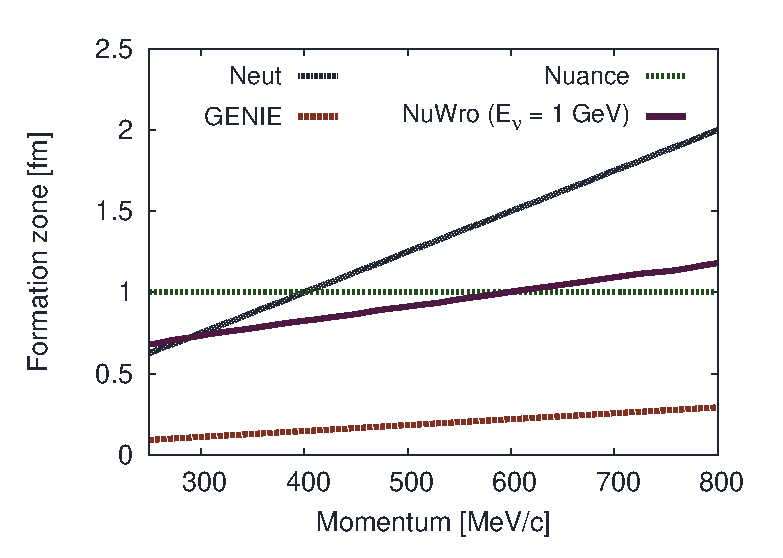
\includegraphics[width = \columnwidth]{img/fzn.eps}
 }
 {
 {\centering Formation time for pions\\}\mbox{}\\
 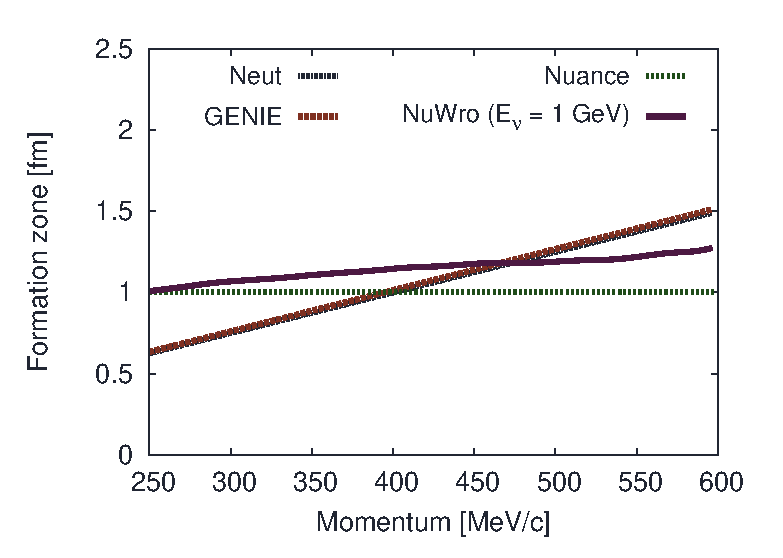
\includegraphics[width = \columnwidth]{img/fzp.eps} 
 }
 
 \begin{itemize}
 
  \item NUANCE uses constant formation length $x = 1$~fm.
  
  \item NEUT uses SKAT parametrization ($\mu^2 = 0.08 \pm 0.04\mbox{ GeV}^2$): \vspace{-5pt}$$x = \frac{|\vec p|}{\mu^2}$$\vspace{-25pt}
 
  \item GENIE uses Rantf  parametrization (assuming transverse momentum $p_T = 0$): \vspace{-15pt}$$x = \tau_0 \frac{E}{M} = \tau_0 \gamma$$
  
 \end{itemize}
 
\end{slide}

\begin{slide}{Form factors}
 \vspace{-10pt}
 \onslide*{1}
 {
    $$\Gamma^\mu_{CC}(q) = \gamma^\mu {\color{pdcolor4}F_1^V (Q^2)} + \frac{i\sigma^{\mu\nu}q_\nu}{2M} {\color{pdcolor4}F_2^V (Q^2)} - \gamma^\mu\gamma_5 {\color{pdcolor5}G_A (Q^2)} - q^\mu\gamma_5 \frac{{\color{pdcolor6}F_P(Q^2)}}{2M}$$
    
    \begin{itemize}
     
     \item Vector form factors are expressed by electromagnetic form factors {\it(Conserved Vector Current - CVC)}: 
     
     $${\color{pdcolor4}F_{1,2}^V(Q^2)} = F_{1,2}^p(Q^2) - F_{1,2}^n(Q^2)$$
     
     \item Axial form factor is assumed to have a dipole form:
     
     $${\color{pdcolor5}G_A(Q^2)} = \frac{g_A}{\left(1 + Q^2/M_A^2\right)^2}$$
     
     \item Pseudoscalar form factor is related to the axial one {\it(Partially Conserved Axial Current - PCAC)}:
     
     $${\color{pdcolor6}F_P(Q^2)} = \frac{4M^2}{m_\pi^2 + Q^2}G_A(Q^2)$$
     
    \end{itemize}
 }
 \onslide*{2}
 {
 $$\hspace{-10pt}\Gamma^\mu_{NC, p(n)} = \gamma^\mu {\color{pdcolor4}F_1^{NC, p(n)} (Q^2)} + \frac{i\sigma^{\mu\nu}q_\nu}{2M} {\color{pdcolor4}F_2^{NC, p(n)} (Q^2)} - \gamma^\mu\gamma_5 {\color{pdcolor5}G_A^{NC, p(n)} (Q^2)}$$
 
 \begin{itemize}
  
     \item Vector form factors are expressed by electromagnetic form factors {\it(Conserved Vector Current - CVC)}: 
     {\footnotesize\vspace{10pt}
     $$\hspace{-20pt}{\color{pdcolor4}F_{1,2}^{NC, p(n)}(Q^2)} = \pm\frac{1}{2}\left(F_{1,2}^p(Q^2) - F_{1,2}^n(Q^2)\right) - 2\sin^2\theta_WF_{1,2}^{p(n)}(Q^2) - \frac{1}{2}F_{1,2}^s(Q^2)$$
     }
     \item Axial form factor is assumed to have a dipole form:
     
     $${\color{pdcolor5}G_A^{NC,p(n)}(Q^2)} = \pm\frac{1}{2}G_A(Q^2) - \frac{1}{2}{\color{pdcolor6}G_A^s(Q^2)}$$
 
    \item The axial strange form factor is assumed to have a dipole form:
    
     $${\color{pdcolor6}G_A^s(Q^2)} = \frac{g_A^s}{\left(1 + Q^2/M_A^2\right)^2}$$
     
 \end{itemize}
 }

 
\end{slide}

\begin{slide}[toc= TE model]{Transverse Enhancement model}
 
 \begin{itemize}
  
  \vspace{10pt}
  \item In the Transverse Enhancement model the two body current contribution is introduced by the modification of the vector magnetic form factors:
  
  $$G^{p,n}_M \rightarrow \tilde G^{p,n}_M = \sqrt{1 + AQ^2\exp{\left(-\frac{Q^2}{B}\right)}}G^{p,n}_M(Q^2)$$
  
  \item $A, B$ are established from the electron data.
  
  \item The cross section for $np-nh$ can be obtained by taking the difference:
  
  $$\frac{\mbox{d}^2\sigma^{np-nh}}{\mbox{d}q\mbox{d}\omega} \equiv \frac{\mbox{d}^2\sigma^{QEL}}{\mbox{d}q\mbox{d}\omega}(\tilde G^{p,n}_M) - \frac{\mbox{d}^2\sigma^{QEL}}{\mbox{d}q\mbox{d}\omega}(G^{p,n}_M)$$
  
  \item The disadvantage of the model is lepton kinematics (``copied'' from the QEL scattering).
 
 \end{itemize}
 
\end{slide}

%%%%% CASCADE ALGORITHM %%%%%

\begin{wideslide}[toc=Cascade algorithm]{The algorithm for intranuclear cascade}

  \rput(0.8\slidewidth, -0.3\slideheight)
  {
  \begin{pspicture}
  
    \onslide*{1-8}
    {
    \psframe[linewidth = 0.025, linecolor = pdcolor1](0,6)(3,7.5)
    \rput[c](1.5,7){\color{pdcolor1}\footnotesize Calculate:}
    \rput[c](1.5,6.5){\color{pdcolor1}\footnotesize $\tilde\lambda(r) = \left[\sigma\rho(r)\right]^{-1}$}
    }
    \onslide*{2-8}
    {
    \psline[linewidth = 0.025, linecolor = pdcolor1]{->}(3,6.75)(3.5,6.75)
    \psframe[linewidth = 0.025, linecolor = pdcolor1](3.5,6)(6.5,7.5)
    \rput[c](5,7){\color{pdcolor1}\footnotesize $\lambda = \tilde\lambda\cdot\ln(P)$}
    \rput[c](5,6.5){\color{pdcolor1}\footnotesize $P = \mbox{rand}[0,1]$}
    }
    \onslide*{3-8}
    {
    \psline[linewidth = 0.025, linecolor = pdcolor1]{->}(5,6)(5,5.5)
    \psframe[linewidth = 0.025, linecolor = pdcolor1](3.5,4)(6.5,5.5)
    \rput[c](5,5){\color{pdcolor1}\footnotesize move particle by}
    \rput[c](5,4.5){\color{pdcolor1}\footnotesize $\mbox{min}(\lambda,\lambda_{max})$}
    }
    \onslide*{4-8}
    {
    \psline[linewidth = 0.025, linecolor = pdcolor1]{->}(3.5,4.75)(3,4.75)
    \psframe[linewidth = 0.025, linecolor = pdcolor1](0,4)(3,5.5)
    \rput[c](1.5,5){\color{pdcolor1}\footnotesize Check $r' > R$}
    \rput[c](1.5,4.5){\color{pdcolor1}\footnotesize $R$ - nucleus radius}
    }
    \onslide*{5-8}
    {
    \psline[linewidth = 0.025, linecolor = pdcolor1]{->}(1.5,4)(1.5,3.5)
    \rput[l](1.6,3.75){\color{pdcolor1}\footnotesize Yes}
    \psframe[linewidth = 0.025, linecolor = pdcolor1](0,2)(3,3.5)
    \rput[c](1.5,3){\color{pdcolor1}\footnotesize The particle}
    \rput[c](1.5,2.5){\color{pdcolor1}\footnotesize leaves nucleus.}
    }
    \onslide*{6-8}
    {
    \psline[linewidth = 0.025, linecolor = pdcolor1]{->}(3,4)(3.5,3.5)
    \rput[l](3.25,3.85){\color{pdcolor1}\footnotesize No}
    \psframe[linewidth = 0.025, linecolor = pdcolor1](3.5,2)(6.5,3.5)
    \rput[c](5,3){\color{pdcolor1}\footnotesize Check}
    \rput[c](5,2.5){\color{pdcolor1}\footnotesize $\lambda < \lambda_{max}$.}
    \psline[linewidth = 0.025, linecolor = pdcolor1](6.5,2.75)(7,2.75)
    \psline[linewidth = 0.025, linecolor = pdcolor1](7,2.75)(7,8)
    \psline[linewidth = 0.025, linecolor = pdcolor1](7,8)(1.5,8)
    \psline[linewidth = 0.025, linecolor = pdcolor1]{->}(1.5,8)(1.5,7.5)
    \rput[l](6.6,2.6){\color{pdcolor1}\footnotesize No}
    }
    \onslide*{7-8}
    {
    \psline[linewidth = 0.025, linecolor = pdcolor1]{->}(5,2)(5,1.5)
    \rput[l](5.1,1.75){\color{pdcolor1}\footnotesize Yes}
    \psframe[linewidth = 0.025, linecolor = pdcolor1](3.5,0)(6.5,1.5)   
    \rput[c](5,1){\color{pdcolor1}\footnotesize Generate}
    \rput[c](5,0.5){\color{pdcolor1}\footnotesize the interaction.}
    }
    \onslide*{8}
    {
    \psframe[linewidth = 0.025, linecolor = pdcolor1](0,0)(3,1.5)
    \rput[c](1.5,1){\color{pdcolor1}\footnotesize Check}
    \rput[c](1.5,0.5){\color{pdcolor1}\footnotesize Pauli blocking.}
    
    \psline[linewidth = 0.025, linecolor = pdcolor1]{->}(3.5,0.75)(3,0.75)
    
    \psline[linewidth = 0.025, linecolor = pdcolor1](0,0.75)(-0.5,0.75)
    \psline[linewidth = 0.025, linecolor = pdcolor1](-0.5,0.75)(-0.5,6.75)
    \psline[linewidth = 0.025, linecolor = pdcolor1]{->}(-0.5,6.75)(0,6.75)    
    }
    
  \end{pspicture}
  }
  
  \rput(0.55\slidewidth, 0.1\slideheight)
  {
  \begin{pspicture}
  
    \onslide*{1-8}
    {
    \pscircle[linewidth = 0.05, linecolor = pdcolor1](0,0){2}

    \pscircle[linestyle = none, fillstyle = solid, fillcolor = pdcolor1](0.75,1){0.2}
    \pscircle[linestyle = none, fillstyle = solid, fillcolor = pdcolor1](-0.5,1.25){0.2}
    \pscircle[linestyle = none, fillstyle = solid, fillcolor = pdcolor1](-1,0){0.2}
    \pscircle[linestyle = none, fillstyle = solid, fillcolor = pdcolor1](0,0.45){0.2}
    \pscircle[linestyle = none, fillstyle = solid, fillcolor = pdcolor1](0.6, -0.75){0.2}
    \pscircle[linestyle = none, fillstyle = solid, fillcolor = pdcolor1](-0.4, -1.2){0.2}
    \pscircle[linestyle = none, fillstyle = solid, fillcolor = pdcolor1](1.25, 0){0.2}
    }

    \onslide*{1-2}
    {
    \pscircle[linestyle = none, fillstyle = solid, fillcolor = pdcolor4](-0.6,-0.6){0.2}
    }

    \onslide*{1}
    {
    \psline[linewidth = 0.02, linecolor = pdcolor1]{<->}(0,0)(-0.4,-0.4)
    \rput[c]{45}(-0.25,-0.1){\color{pdcolor1}\footnotesize $r$}
    }

    \onslide*{7}
    {
    \psline[linewidth = 0.02, linecolor = pdcolor3]{|<->|}(-0.38,-0.73)(1,-0.1)    
    \rput[c]{25}(0.2,-0.6){\color{pdcolor3}\tiny $x_{max}$}
    }
    
    \onslide*{7-8}
    {
    \pscircle[linestyle = none, fillstyle = solid, fillcolor = pdcolor5](0.8,0.15){0.2}    
    \psline[linewidth = 0.02, linecolor = pdcolor5]{->}(1,0.275)(1.2,0.375)
    \pscircle[linestyle = none, fillstyle = solid, fillcolor = pdcolor1](0.5,0.15){0.2}    
    \psline[linewidth = 0.02, linecolor = pdcolor1]{->}(0.5,0.375)(0.5,0.575)
    }
    
    \onslide*{8}
    {
    \psline[linewidth = 0.02, linecolor = pdcolor1]{->}(0.75, 1.225)(0.75, 1.435)
    \pscircle[linewidth = 0.01, linecolor = pdcolor4](0.75, 1.325){0.125}
    \pscircle[linewidth = 0.01, linecolor = pdcolor4](0.5, 0.475){0.125}
    }
    
    \onslide*{2-4,6-8}
    {
    \psline[linewidth = 0.02, linecolor = pdcolor4]{->}(-0.4,-0.55)(0.4,-0.2)
    }
    
    \onslide*{3-4,6-8}
    {
    \pscircle[linestyle = none, fillstyle = solid, fillcolor = pdcolor4,opacity = 0.5](-0.6,-0.6){0.2}
    \pscircle[linestyle = none, fillstyle = solid, fillcolor = pdcolor4](0.6,-0.1){0.2}
    }
    
    \onslide*{4}
    {
    \psline[linewidth = 0.02, linecolor = pdcolor1]{<->}(0,0)(0.4,-0.1)
    \rput[c]{-10}(0.3,0.1){\color{pdcolor1}\footnotesize $r'$}
    }

    \onslide*{5}
    {
    \psline[linewidth = 0.02, linecolor = pdcolor4]{->}(-0.8,-0.675)(-1.8,-1.2)
    \pscircle[linestyle = none, fillstyle = solid, fillcolor = pdcolor4,opacity = 0.5](-0.6,-0.6){0.2}
    \pscircle[linestyle = none, fillstyle = solid, fillcolor = pdcolor4](-2,-1.3){0.2}
    }
    
    \onslide*{6}
    {
    \psline[linewidth = 0.02, linecolor = pdcolor3]{|<->|}(-0.38,-0.73)(0.3,-0.425)    
    \rput[c]{25}(0,-0.7){\color{pdcolor3}\tiny $x_{max}$}
    }
    
  \end{pspicture}
  }

\end{wideslide}